\documentclass[article, 1.5space, letterpaper, 12pt, oneside, header, footer]{SydeClass}
\graphicspath{{images/}}
\usepackage{subfigure}
\usepackage{eqnarray}


% --------- Title Info -----------
\titlestyle{design} % used in SydeTitle.tex. Can equal one of the following values: design, work

\title{Lab 2}
\subtitle{Image Enhancement and Restoration}

\coursecode{SYDE 475}
\department{Systems Design Engineering}

\author{Colin Heics, 20240543}
\authorheader{C. Heics}
\authortwo{Neil Sokol, 20265064}
\authorheadertwo{N. Sokol}

\date{\today}
\instructor{Alex Wong}

\subsectionfont{\normalsize}
\setcounter{secnumdepth}{2}
\setcounter{tocdepth}{1}

\usepackage{listings}
\usepackage{color}
\usepackage{textcomp}
\definecolor{listinggray}{gray}{0.9}
\definecolor{lbcolor}{rgb}{0.9,0.9,0.9}
\lstset{
	backgroundcolor=\color{lbcolor},
	tabsize=4,
	rulecolor=,
	language=matlab,
        basicstyle=\scriptsize,
        upquote=true,
        aboveskip={1.5\baselineskip},
        columns=fixed,
        showstringspaces=false,
        extendedchars=true,
        breaklines=true,
        prebreak = \raisebox{0ex}[0ex][0ex]{\ensuremath{\hookleftarrow}},
        frame=single,
        showtabs=false,
        showspaces=false,
        showstringspaces=false,
        identifierstyle=\ttfamily,
        keywordstyle=\color[rgb]{0,0,1},
        commentstyle=\color[rgb]{0.133,0.545,0.133},
        stringstyle=\color[rgb]{0.627,0.126,0.941},
}

% ############  ############
\begin{document}

% ---------- Title ------------

%% Use the command "
%% Use the command "
%% Use the command "\input{SydeTitle}" in your main file to include this file.

\begin{titlepage}
	\makeatletter % use .cls usage for <at>
	
	\pagestyle{empty}
	\equalmargins
	
	\ifthenelse{\equal{\@titlestyle}{work}}{
		\begin{center}
			\vspace*{2em}

			University of Waterloo\\
			Faculty of Engineering\\
			Department of Systems Design Engineering

			\null\vfill
		
			\Huge\@title \\
			\ifdefined \@subtitle \Large\@subtitle \\ \fi
			\normalsize

			\null\vfill
		
			\@company\\
			\@companyaddress \vspace{2em}
		
			\@author\\
			\@date
		\end{center}
	}{\relax} % end if
	
	\ifthenelse{\equal{\@titlestyle}{design}}{
		\begin{center}
			\vspace*{5em}
	
			\Huge\@title \\
			\ifdefined \@subtitle \Large\@subtitle \\ \fi
			\normalsize
	
			\vfill
		
			A Report Submitted in Partial Fulfilment\\
			of the Requirements for \@coursecode \vspace{4em}
		
			\ifdefined \@groupname \@groupname \\ \fi
		  \@author \\
			\ifdefined \@authortwo \@authortwo \\ \fi
			\ifdefined \@authorthree \@authorthree \\ \fi
			\ifdefined \@authorfour \@authorfour \\ \fi
		  \vspace{3em}
		
			Faculty of Engineering \\
			\ifdefined \@department Department of \@department \\ \fi
			\vspace{3em}
		
			\@date \\
			
			\ifdefined \@instructor Course Instructor: \@instructor \\ \fi
			\ifdefined \@supervisor Project Supervisor: \@supervisor \\ \fi
			
		\end{center}
	}{\relax} % end if
	
	\makeatother % return to document usage for <at>
\end{titlepage}

%\pagestyle{plain}
%\offsetmargins" in your main file to include this file.

\begin{titlepage}
	\makeatletter % use .cls usage for <at>
	
	\pagestyle{empty}
	\equalmargins
	
	\ifthenelse{\equal{\@titlestyle}{work}}{
		\begin{center}
			\vspace*{2em}

			University of Waterloo\\
			Faculty of Engineering\\
			Department of Systems Design Engineering

			\null\vfill
		
			\Huge\@title \\
			\ifdefined \@subtitle \Large\@subtitle \\ \fi
			\normalsize

			\null\vfill
		
			\@company\\
			\@companyaddress \vspace{2em}
		
			\@author\\
			\@date
		\end{center}
	}{\relax} % end if
	
	\ifthenelse{\equal{\@titlestyle}{design}}{
		\begin{center}
			\vspace*{5em}
	
			\Huge\@title \\
			\ifdefined \@subtitle \Large\@subtitle \\ \fi
			\normalsize
	
			\vfill
		
			A Report Submitted in Partial Fulfilment\\
			of the Requirements for \@coursecode \vspace{4em}
		
			\ifdefined \@groupname \@groupname \\ \fi
		  \@author \\
			\ifdefined \@authortwo \@authortwo \\ \fi
			\ifdefined \@authorthree \@authorthree \\ \fi
			\ifdefined \@authorfour \@authorfour \\ \fi
		  \vspace{3em}
		
			Faculty of Engineering \\
			\ifdefined \@department Department of \@department \\ \fi
			\vspace{3em}
		
			\@date \\
			
			\ifdefined \@instructor Course Instructor: \@instructor \\ \fi
			\ifdefined \@supervisor Project Supervisor: \@supervisor \\ \fi
			
		\end{center}
	}{\relax} % end if
	
	\makeatother % return to document usage for <at>
\end{titlepage}

%\pagestyle{plain}
%\offsetmargins" in your main file to include this file.

\begin{titlepage}
	\makeatletter % use .cls usage for <at>
	
	\pagestyle{empty}
	\equalmargins
	
	\ifthenelse{\equal{\@titlestyle}{work}}{
		\begin{center}
			\vspace*{2em}

			University of Waterloo\\
			Faculty of Engineering\\
			Department of Systems Design Engineering

			\null\vfill
		
			\Huge\@title \\
			\ifdefined \@subtitle \Large\@subtitle \\ \fi
			\normalsize

			\null\vfill
		
			\@company\\
			\@companyaddress \vspace{2em}
		
			\@author\\
			\@date
		\end{center}
	}{\relax} % end if
	
	\ifthenelse{\equal{\@titlestyle}{design}}{
		\begin{center}
			\vspace*{5em}
	
			\Huge\@title \\
			\ifdefined \@subtitle \Large\@subtitle \\ \fi
			\normalsize
	
			\vfill
		
			A Report Submitted in Partial Fulfilment\\
			of the Requirements for \@coursecode \vspace{4em}
		
			\ifdefined \@groupname \@groupname \\ \fi
		  \@author \\
			\ifdefined \@authortwo \@authortwo \\ \fi
			\ifdefined \@authorthree \@authorthree \\ \fi
			\ifdefined \@authorfour \@authorfour \\ \fi
		  \vspace{3em}
		
			Faculty of Engineering \\
			\ifdefined \@department Department of \@department \\ \fi
			\vspace{3em}
		
			\@date \\
			
			\ifdefined \@instructor Course Instructor: \@instructor \\ \fi
			\ifdefined \@supervisor Project Supervisor: \@supervisor \\ \fi
			
		\end{center}
	}{\relax} % end if
	
	\makeatother % return to document usage for <at>
\end{titlepage}

%\pagestyle{plain}
%\offsetmargins

% ############ Chapters ############
\pagenumbering{arabic}

\section{Noise Generation}

When evaluating image processing algorithms, it is important to see how they perform under various levels of noise.


\begin{figure}[ht]
\centering
	\subfigure[Original image]{
	
\includegraphics[width=0.45\linewidth]{question2/toy}
	}
\end{figure}

\begin{figure}[ht]
\centering
	\subfigure[Image with Gaussian Noise; $\sigma^2$=0.01]{
	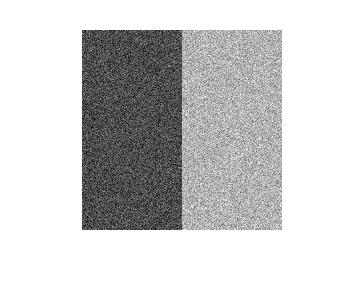
\includegraphics[width=0.45\linewidth]{question2/gauss}
	}
	\subfigure[Histogram of Gaussian Noise Image]{
	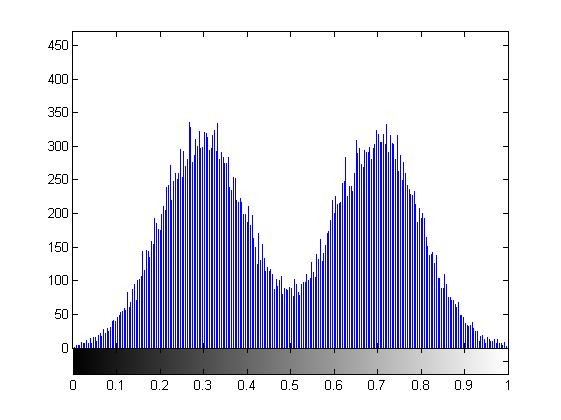
\includegraphics[width=0.45\linewidth]{question2/gauss_hist}
	}
	\subfigure[Image with Speckle Noise; $\sigma^2$=0.04]{
	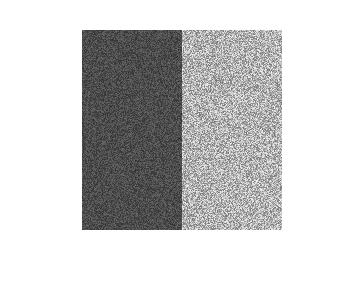
\includegraphics[width=0.45\linewidth]{question2/speckle}
	}
	\subfigure[Histogram of Speckle Noise Image]{
	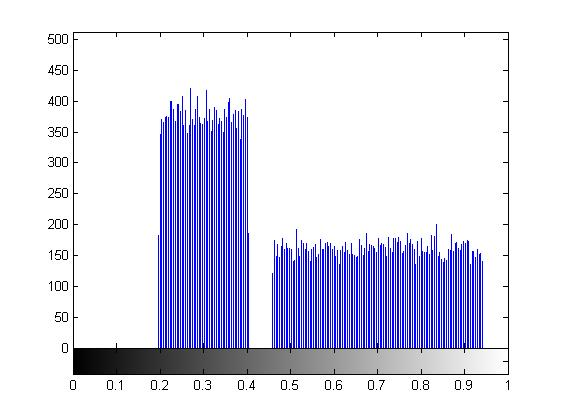
\includegraphics[width=0.45\linewidth]{question2/speckle_hist}
	}
	\subfigure[Image with Salt and Pepper Noise; $\rho$=0.05]{
	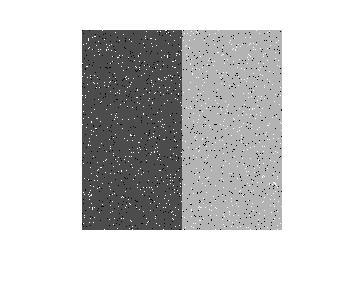
\includegraphics[width=0.45\linewidth]{question2/salt}
	}
	\subfigure[Histogram of Salt and Pepper Image]{
	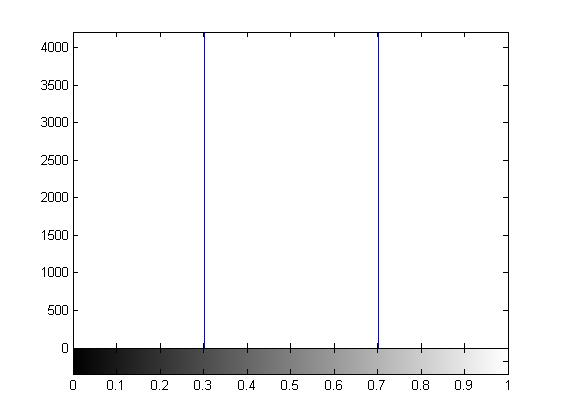
\includegraphics[width=0.45\linewidth]{question2/salt_hist}
	}
	\caption{Toy image with Gaussian, Salt and Pepper, and Speckle Noise}
	\label{fig:noiseGeneration.toy}
\end{figure}
 

\subsection{Discussion questions}

\subsubsection{ Describe each of the histograms in the context of the corresponding noise models. Why do they appear
that way?}
In the Gaussian histogram, image intensities are grouped in Gaussian distributions centred around the two intensity values of the original image. It appears the way it is because as additive noise, all that is being done is the Gaussian distribution is added to the image. Speckled noise, which is multiplicative, appears to be a flat distribution centred around the original intensities. There is more variance around the higher original intensity value, which is due to the multiplicative nature of speckle noise.

\subsubsection{Are there visual differences between the noise contaminated images? What are they? Why}
There are some visual differences. The Gaussian has a lot more extra bright or extra dark pixels, while speckled has more that are more off by a smaller intensity. This is because the Gaussian is additive noise, and the speckled is multiplicative.

\subsubsection{In the speckle noise case, what is the underlying distribution used? Can you tell from the histogram?
How?}
The underlying distribution is uniform. You can tell from the histogram because the intensities are distributed roughly evenly (i.e. same number of pixels). 

\subsubsection{In the speckle noise case, you will notice that the peaks of the histogram are no longer of the same
height as they were in the original image. Also, the spread around each of the peaks is also different
from each other. Why? Hint: Noise is multiplicative}
Since the noise is multiplicative, it is proportional to the local grey level in the image. i.e. there will be a wider spread of values around higher grey levels, as we can see with the right-most spread having a higher variance.



\section{Noise Reduction in the Spatial Domain}

\clearpage
\subsection{Section0}
\begin{figure}[ht]
\centering
	\subfigure[Original image]{
	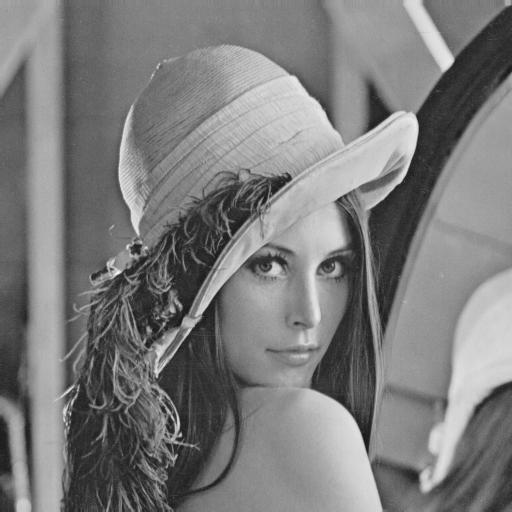
\includegraphics[width=0.45\linewidth]{question3/0_lenaBase}
	}
	\subfigure[Histogram]{
	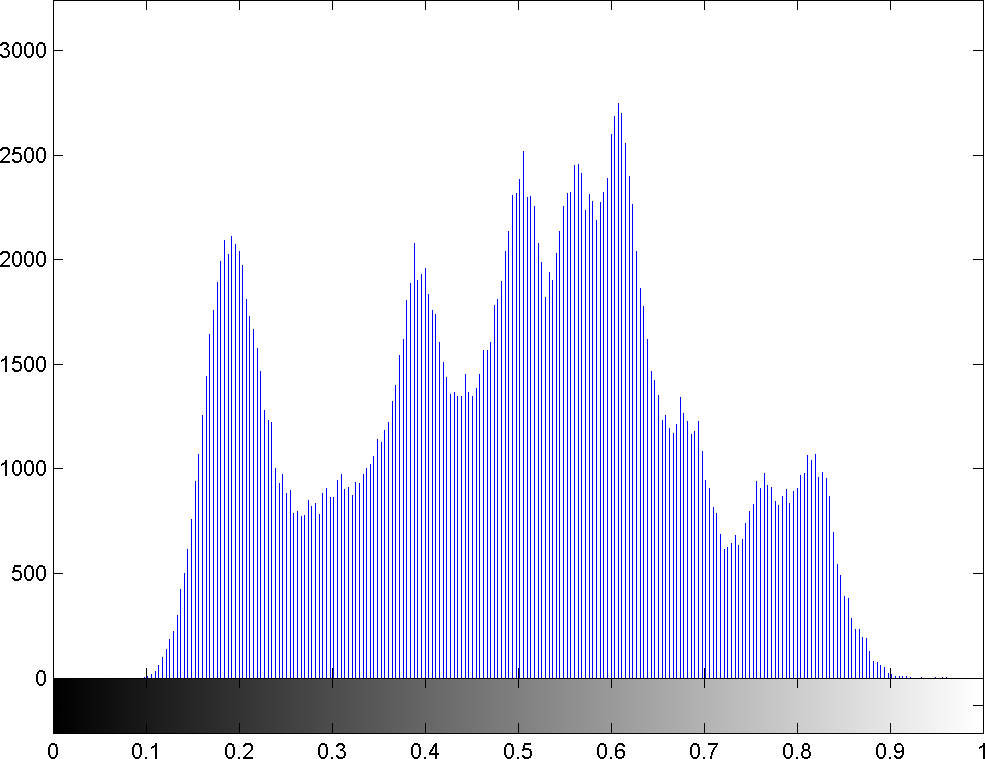
\includegraphics[width=0.45\linewidth]{question3/0_lenaBase_hist}
	}
	\subfigure[Image with Gaussian noise $\mu$=0, $\sigma^2$=0.002; PSNR +26.99dB]{
	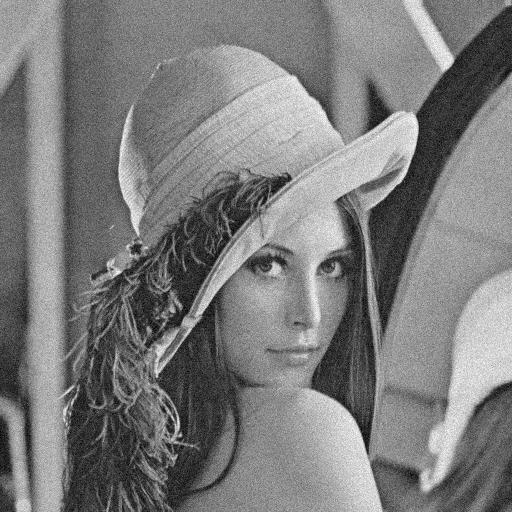
\includegraphics[width=0.45\linewidth]{question3/0_lenaNoisyGauss}
	}
	\subfigure[Histogram]{
	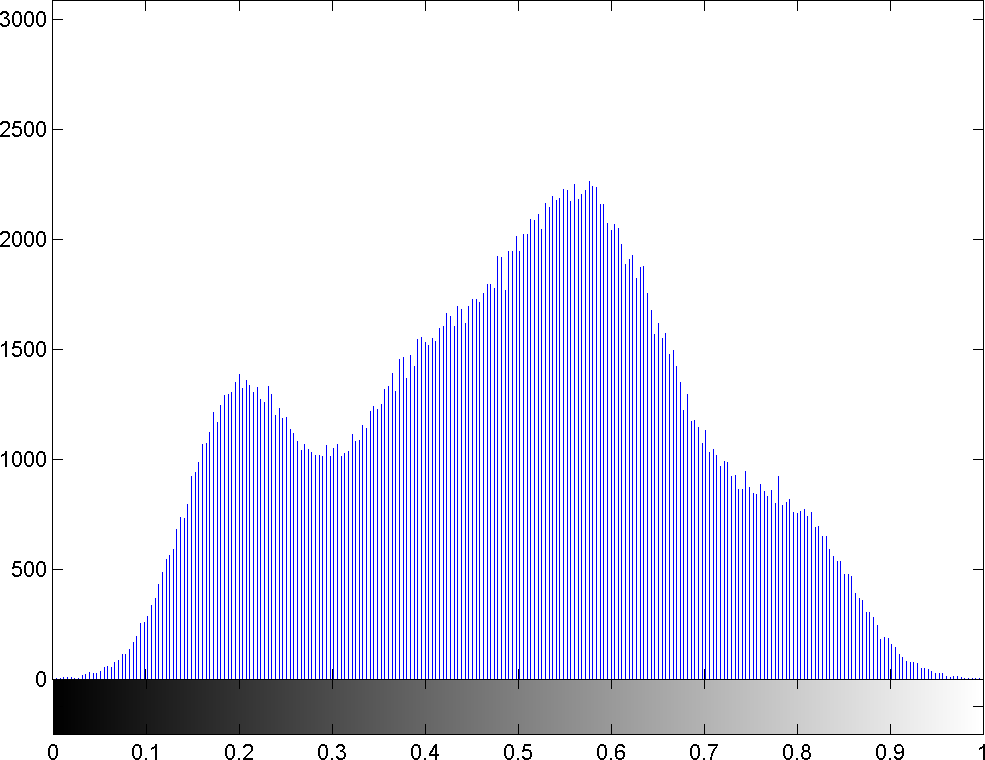
\includegraphics[width=0.45\linewidth]{question3/0_lenaNoisyGauss_hist}
	}
	\caption{Images with Gaussian noise}
	\label{fig:gaussianNoise}
\end{figure}


\clearpage
\subsection{Section1}
\begin{figure}[ht]
\centering
	\subfigure[Denoised image with 3x3 average kernel; PSNR +30.63dB]{
	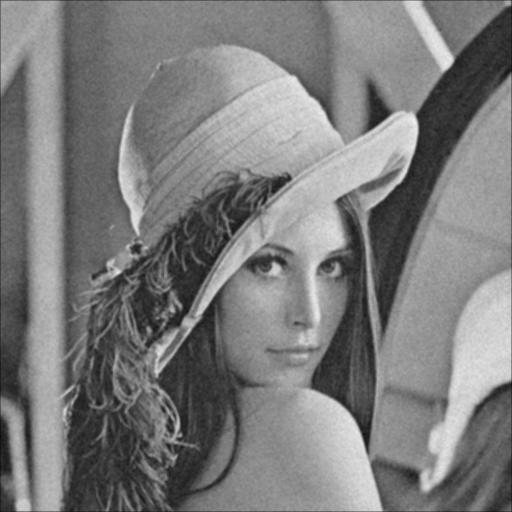
\includegraphics[width=0.45\linewidth]{question3/1_lenaDeNoisyGauss3x3avg}
	}
	\subfigure[Histogram]{
	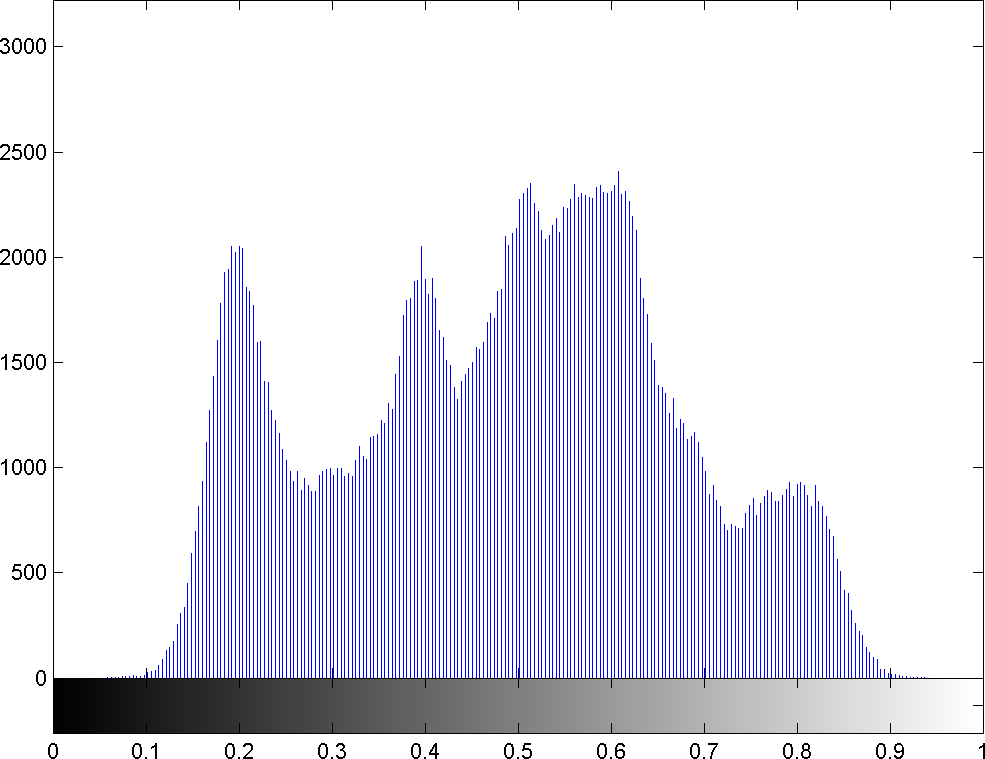
\includegraphics[width=0.45\linewidth]{question3/1_lenaDeNoisyGauss3x3avg_hist}
	}
	
	\caption{Images with Gaussian noise}
	\label{fig:gaussianNoise}
\end{figure}

\clearpage
\subsection{Section2}
\begin{figure}[ht]
\centering
	\subfigure[Denoised image with 7x7 average kernel; PSNR +26.23dB]{
	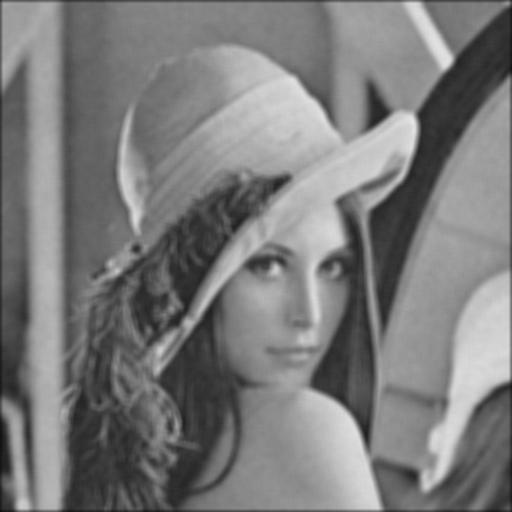
\includegraphics[width=0.45\linewidth]{question3/2_lenaDeNoisyGauss7x7avg}
	}
	\subfigure[Histogram]{
	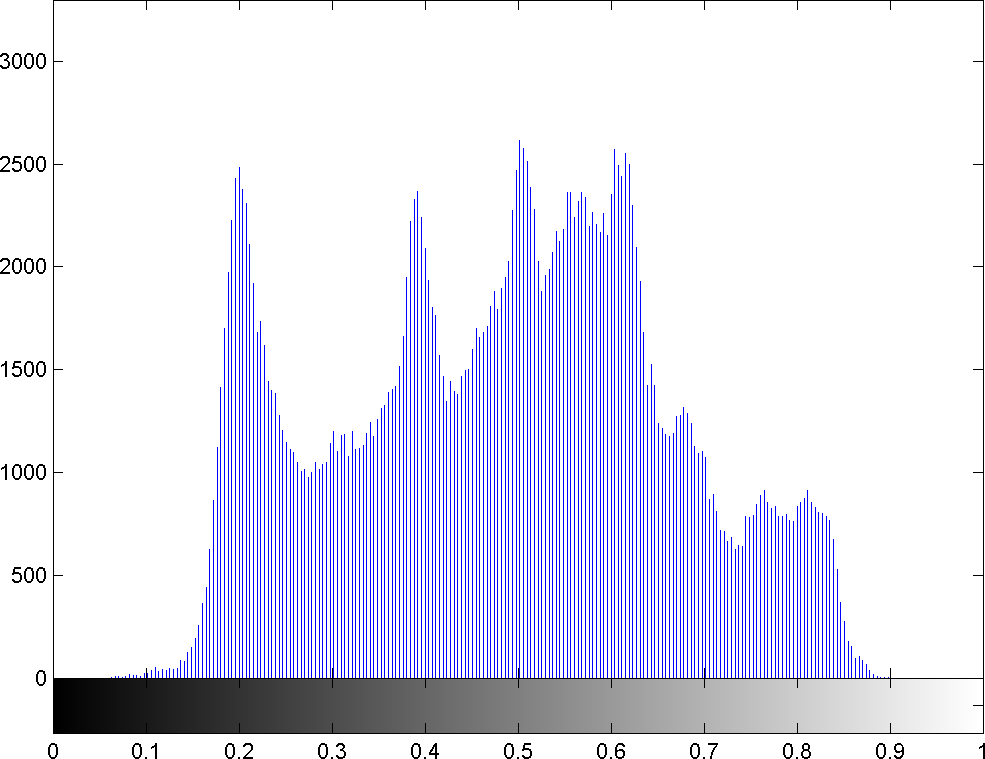
\includegraphics[width=0.45\linewidth]{question3/2_lenaDeNoisyGauss7x7avg_hist}
	}
	
	\caption{Images with Gaussian noise}
	\label{fig:gaussianNoise}
\end{figure}

\clearpage
\subsection{Section3}
\begin{figure}[ht]
\centering
	\subfigure[Denoised image with 7x7 Gaussian kernel; PSNR +30.82dB]{
	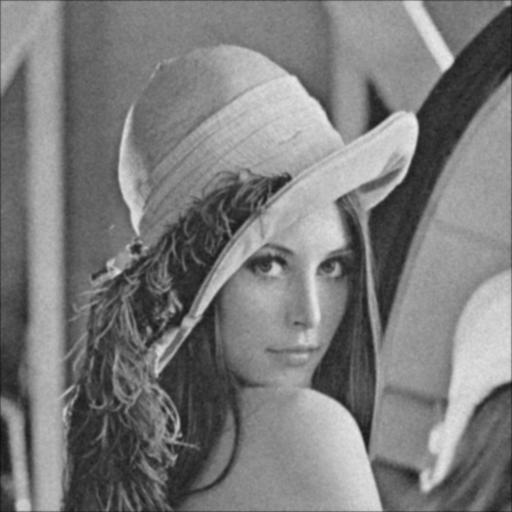
\includegraphics[width=0.45\linewidth]{question3/3_lenaDeNoisyGauss7x7avgGauss}
	}
	\subfigure[Histogram]{
	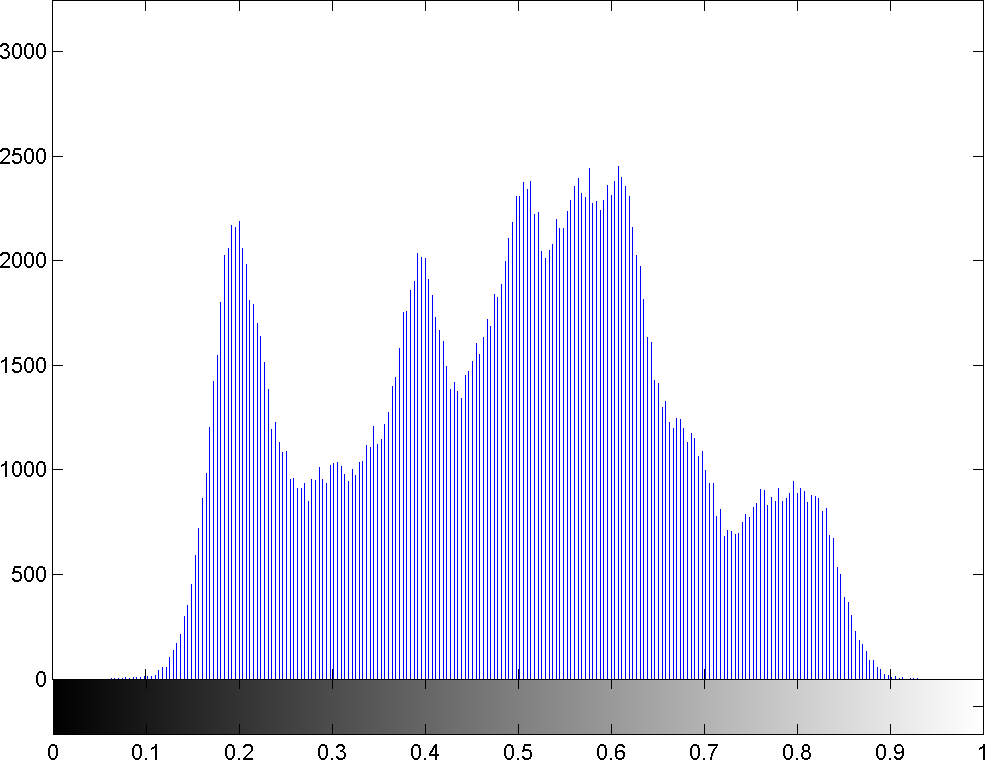
\includegraphics[width=0.45\linewidth]{question3/3_lenaDeNoisyGauss7x7avgGauss_hist}
	}
	
	\caption{Images with Gaussian noise}
	\label{fig:gaussianNoise}
\end{figure}


\clearpage
\subsection{Section4}

\begin{figure}[ht]
\centering
	\subfigure[S\&P noise on original image; PSNR +18.41dB]{
	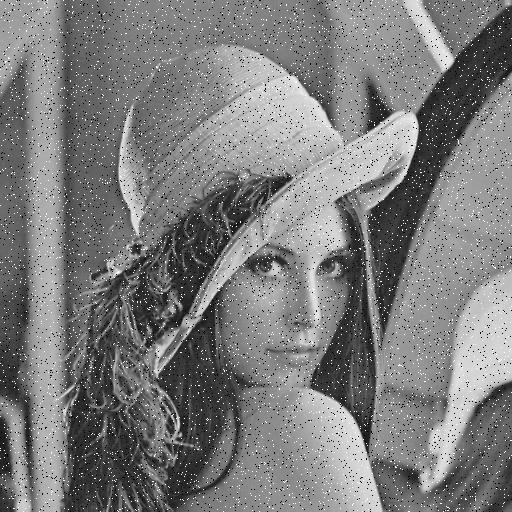
\includegraphics[width=0.45\linewidth]{question3/4_lenaNoisySp}
	}
	\subfigure[Histogram]{
	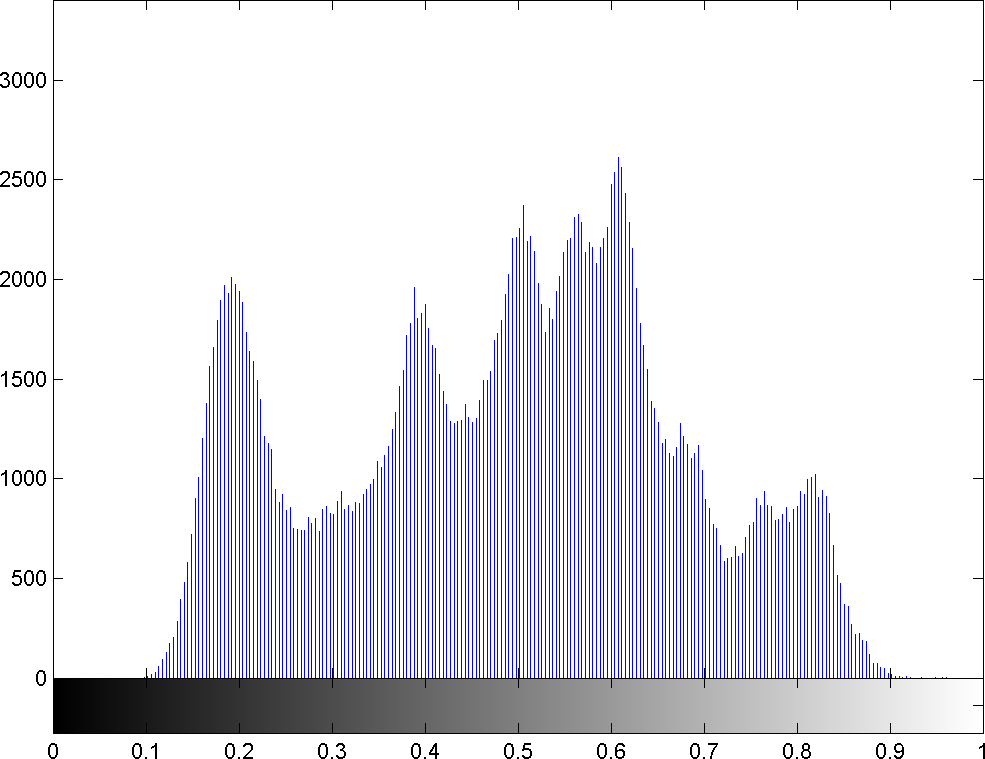
\includegraphics[width=0.45\linewidth]{question3/4_lenaNoisySp_hist}
	}
\end{figure}

\begin{figure}[ht]
\centering	
	\subfigure[S\&P denoised with 7x7 average kernel; PSNR +25.52dB]{
	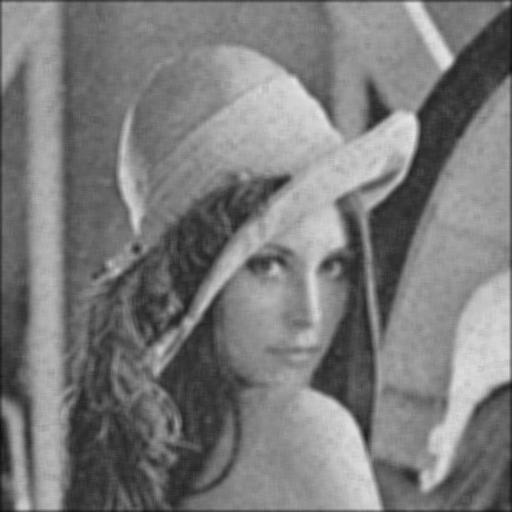
\includegraphics[width=0.45\linewidth]{question3/4_lenaDeNoisySp_7x7Avg}
	}
	\subfigure[Histogram]{
	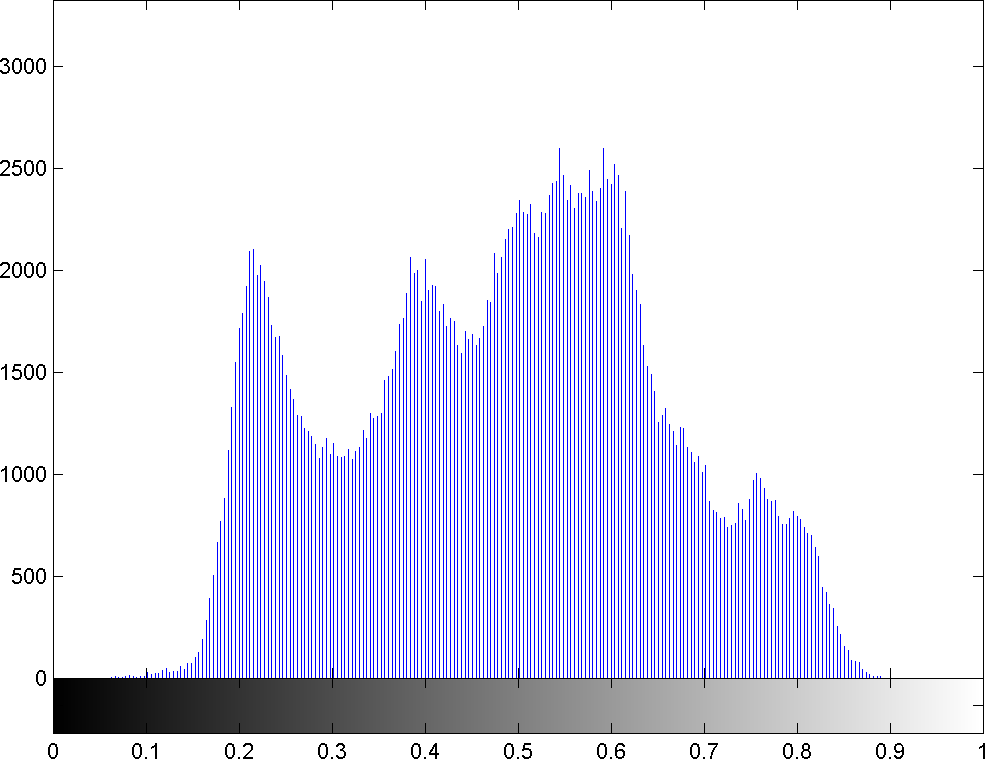
\includegraphics[width=0.45\linewidth]{question3/4_lenaDeNoisySp_7x7Avg_hist}
	}
\end{figure}

\begin{figure}[ht]
\centering
	\subfigure[S\&P denoised with 7x7 Gaussian kernel; PSNR +27.08dB]{
	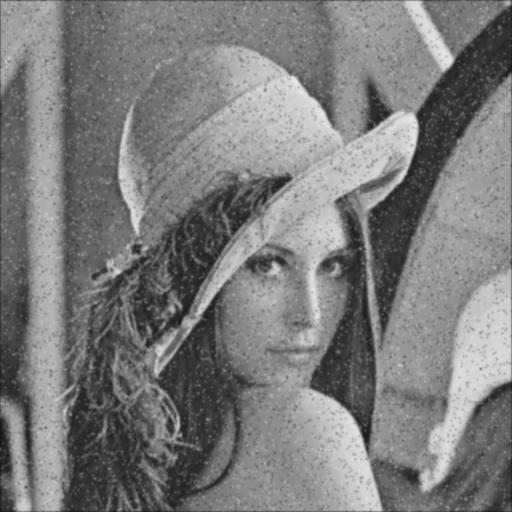
\includegraphics[width=0.45\linewidth]{question3/4_lenaDeNoisySp_7x7AvgGauss}
	}
	\subfigure[Histogram]{
	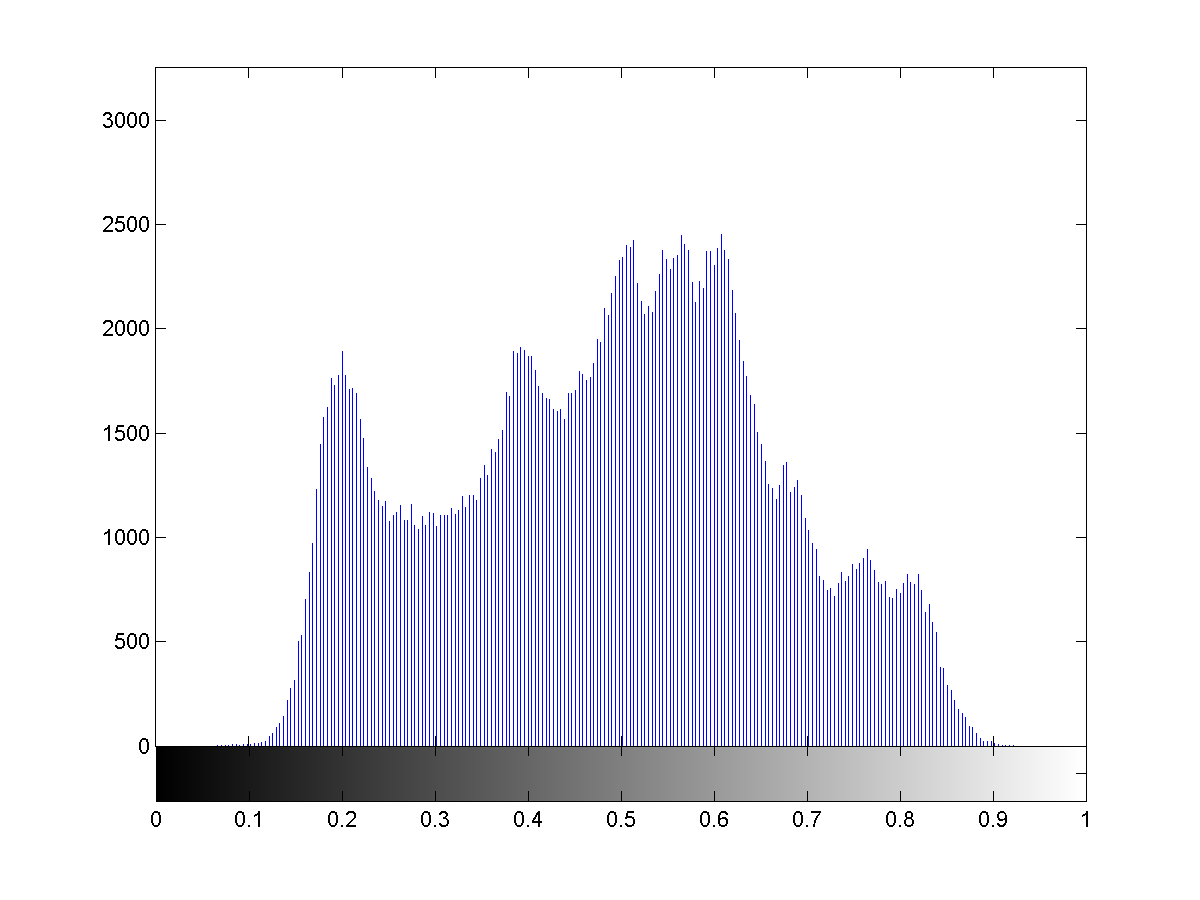
\includegraphics[width=0.45\linewidth]{question3/4_lenaDeNoisySp_7x7AvgGauss_hist}
	}
\end{figure}


\clearpage
\subsection{Section5}

\begin{figure}[ht]
\centering
	\subfigure[S\&P denoised with median filter; PSNR +34.47]{
	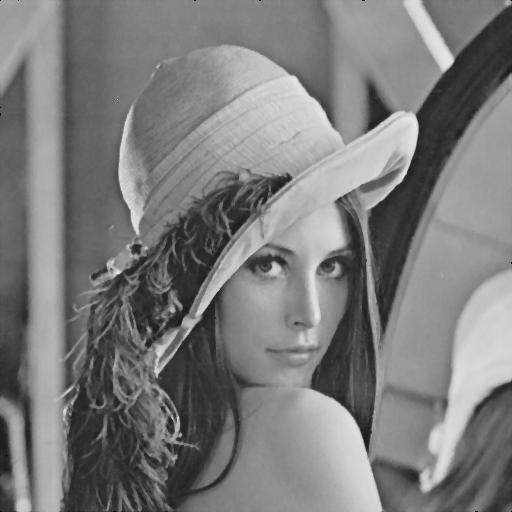
\includegraphics[width=0.45\linewidth]{question3/5_lenaDeNoisyMedian}
	}
	\subfigure[Histogram]{
	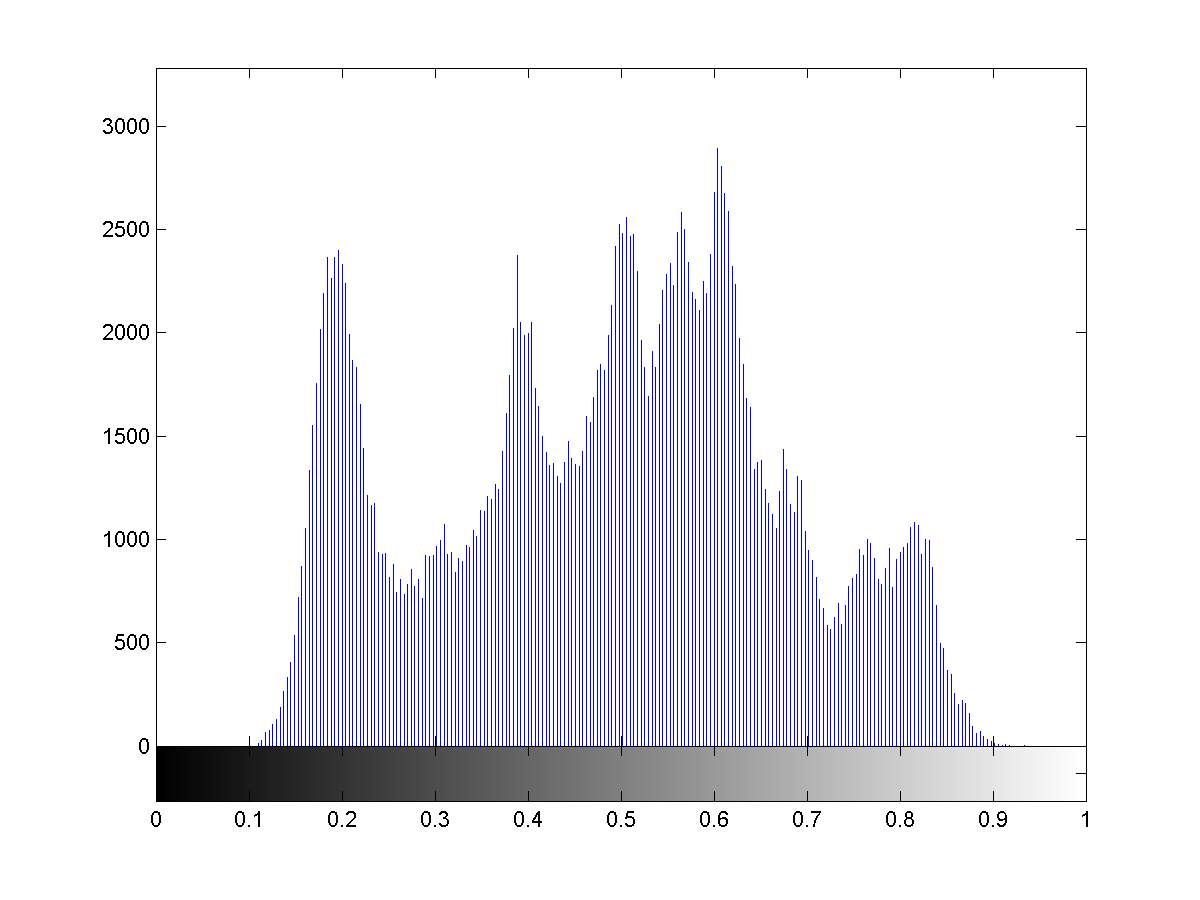
\includegraphics[width=0.45\linewidth]{question3/5_lenaDeNoisyMedian_hist}
	}
\end{figure}

\clearpage


\subsection{Discussion questions}

\subsubsection{Compare the visual difference between the noisy image and the denoised image. How well did it
work? Why? Did the PSNR decrease?}
The denoised image appears blurrier. The denoising worked rather well, as the PSNR is higher in the denoised image. This is because Gaussian is additive noise, and averaging works well at removing additive noise.

\subsubsection{Compare the histograms of the noise-free, noisy, and denoised images. What happened? Why}
The noisy histogram is missing the sharp peaks of the noise free image, instead smoothing it closer to an overall Gaussian distributed shape (due to the additive noise). The averaging filter partially restores this histogram pattern.


\subsubsection{Based on visual quality of the denoised image, what are the benefits and drawbacks associated with
the average filter}
While overall noise is reduced and the PSNR is higher, the image is of reduced visual quality compared to the original (i.e. blurry).


\subsubsection{Compare the visual difference between the denoised image from the 7x7 filtering kernel and the
denoised image from the 3x3 filtering kernel. Are there any differences? Why? Did the PSNR
decrease? Why}
The 7x7 filtered image is even blurrier than the 3x3 filtered one. This is because it averages over a wider area. The PSNR also decreased, with the PSNR now slightly less than that of the noisy image. This is because by taking a wider averaging window, high frequency elements such as edges are further suppressed.


\subsubsection{Compare the histograms of the two denoised images. What are the differences? Why}
The histogram of the 7x7 has sharper peaks than the 3x3, more closely mirroring that of the original noiseless image. This is because


\subsubsection{Based on visual quality of the denoised image, what are the benefits and drawbacks associated with
using a larger window size?}
While the noise is basically gone from the image, it is extremely blurry; many fine details (especially edges) are lost.


\subsubsection{Compare the visual difference between the denoised image from the Gaussian filtering kernel and the
denoised images from the averaging filter kernels. Are there any differences? Why? Did the PSNR
decrease? Why}
The Gaussian filtered image is less blurry than the two averaging filtered images. Finer details are better preserved. This is because with the Gaussian kernel, pixels further away from the centre are weighted less, unlike the uniform averaging of the averaging kernel.


\subsubsection{Compare the histograms of the denoised image using the Gaussian filtering kernel and the denoised
images from the averaging filter kernels. What are the differences? Why?}
<<<<<<< HEAD
The sharp peaks of seen in the 7x7 averaging filter are less pronounced in the Gaussian filter. 
=======
The sharp peaks of seen in the 7x7 averaging filter are less pronounced in the gaussian filter. This is because 
>>>>>>> 5ac6e4450c0815d9bdd673d1c5660bbfedde6aae


\subsubsection{Based on visual quality of the denoised image, what are the benefits and drawbacks associated with
using a Gaussian kernel as opposed to an averaging kernel?}
The Gaussian kernal results in a less blurry image than the averaging kernal.


\subsubsection{How does the averaging filter and Gaussian filtering methods perform on the noisy image in terms of
noise reduction? Explain in terms of visual quality as well as PSNR. Why do we get such results?}


\subsubsection{Compare the histograms of the denoised images with that of the noisy image. What characteristics
are present in all of the histograms? Why?}


\subsubsection{How does the denoised image produced using the median filter compare with the denoised images
produced using averaging filter and Gaussian filtering methods? Explain in terms of visual quality
as well as PSNR. Why do we get such results with median filter when compared to the other spatial
filtering methods?}
The median filter produces a superior quality image compared to the gaussian and averaging filters. The PSNR is also significantly higher. We get such results with the median filter because by taking the median value, excessive high/low intensities due to noise do not get taken into account. With the averaging/gaussian filters, these get averaged into the denoised image.



\section{Sharpening in the spatial domain}

\subsection{Section1}
\begin{figure}[ht]
\centering
	\subfigure[Base Cameraman image]{
	\includegraphics[width=0.45\linewidth]{question4/1_camBase}
	}
	\subfigure[Original image - Blurred image]{
	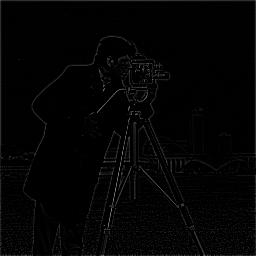
\includegraphics[width=0.45\linewidth]{question4/1_cam_highBoost}
	}
\end{figure}

\subsection{Section2}
\begin{figure}[ht]
\centering
	\subfigure[High-boosted image, A=1.0]{
	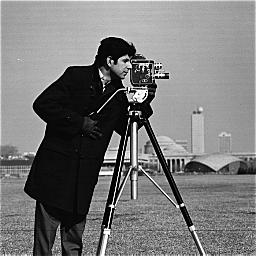
\includegraphics[width=0.45\linewidth]{question4/2_cam_highBoost_10}
	}
\end{figure}


\subsection{Section3}
\begin{figure}[ht]
\centering
	\subfigure[High-boosted image, A=0.5]{
	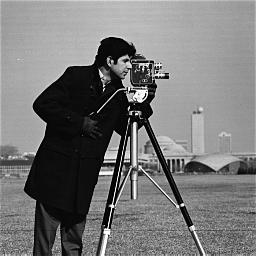
\includegraphics[width=0.45\linewidth]{question4/3_cam_highBoost_05}
	}
\end{figure}

\begin{figure}[ht]
\centering
	\subfigure[High-boosted image, A=1.5]{
	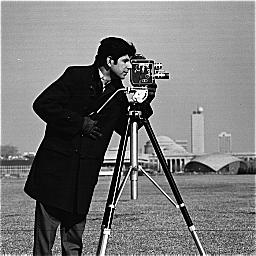
\includegraphics[width=0.45\linewidth]{question4/3_cam_highBoost_15}
	}
	\subfigure[High-boosted image, A=4.0]{
	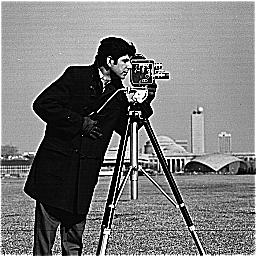
\includegraphics[width=0.45\linewidth]{question4/3_cam_highBoost_40}
	}
\end{figure}




\section{Noise reduction in the frequency domain}

\subsection{Section1}
\begin{figure}[ht]
\centering
	\subfigure[Base Lena image]{
	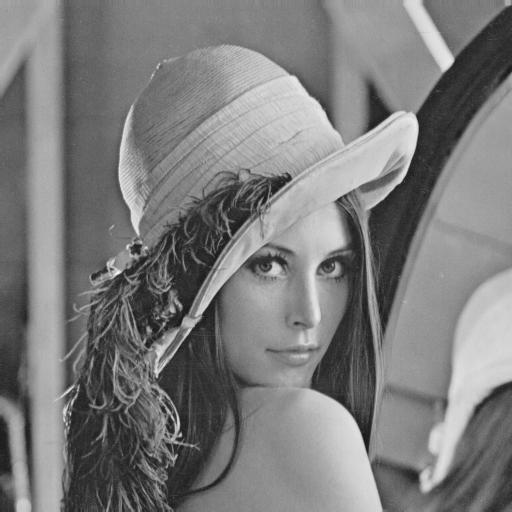
\includegraphics[width=0.45\textwidth]{question5/1_lenaBase}
	}
	\subfigure[Log Fourier Spectrum]{
	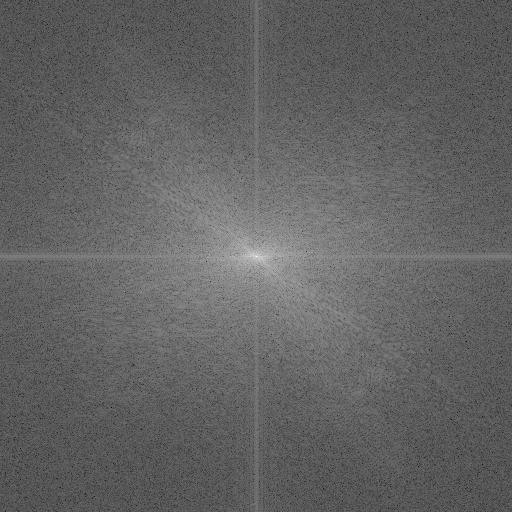
\includegraphics[width=0.45\textwidth]{question5/1_lenaBase_fft}
	}
	\subfigure[Lena image with Gaussian noise, $\sigma^2$=0.005; PSNR +23.02dB]{
	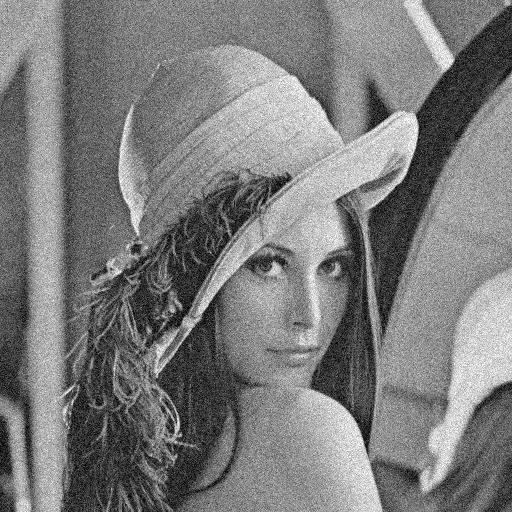
\includegraphics[width=0.45\textwidth]{question5/1_lenaNoisy}
	}
	\subfigure[Log Fourier Spectrum]{
	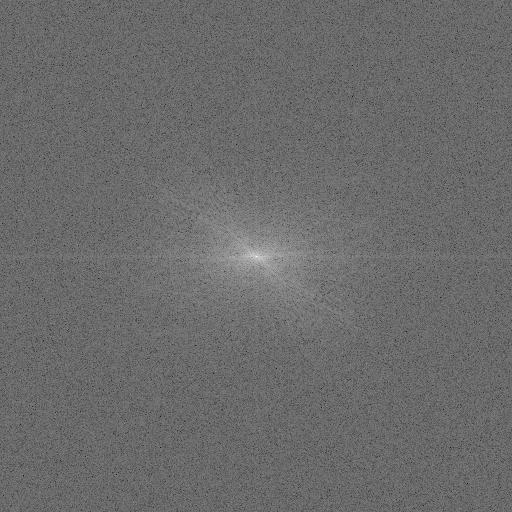
\includegraphics[width=0.45\textwidth]{question5/1_lenaNoisy_fft}
	}
\end{figure}

\subsection{Section2}
\begin{figure}[ht]
\centering
	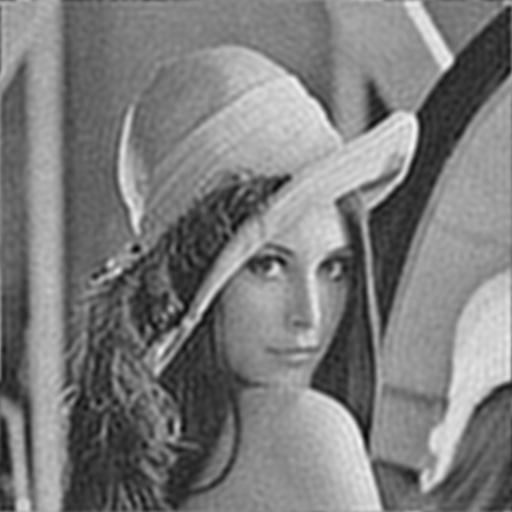
\includegraphics[width=0.45\textwidth]{question5/2_lena_LFP_60}
	\caption{Image filtered using low-pass with a cutoff of 60; PSNR +27.90dB}
\end{figure}

\subsection{Section3}
\begin{figure}[ht]
\centering
	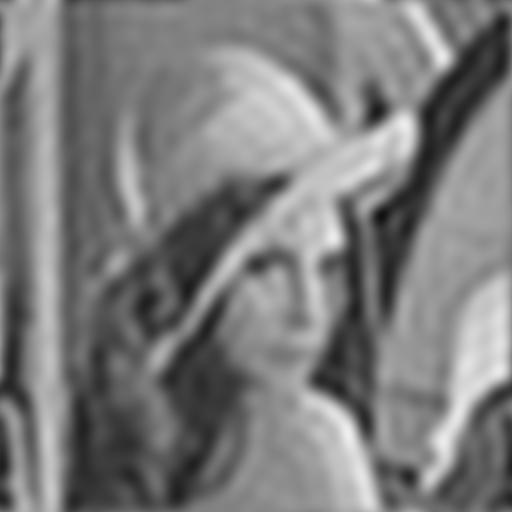
\includegraphics[width=0.45\textwidth]{question5/3_lena_LFP_20}
	\caption{Image filtered using low-pass with a cutoff of 20; PSNR +23.11dB}
\end{figure}

\subsection{Section4}
\begin{figure}[ht]
\centering
	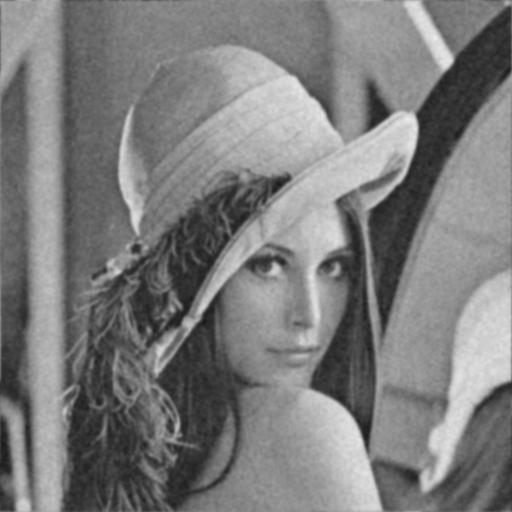
\includegraphics[width=0.45\textwidth]{question5/4_lena_LFP_gauss60}
	\caption{Image filtered using Gaussian low-pass filter, $\sigma^2$=60; PSNR +29.53dB}
\end{figure}

\clearpage
\section{Image reconstruction in the frequency domain}

In the following section, reconstructing an image based on the inverse of the degradation will be examined.

\subsection{Restoring an image with }

\subsubsection{Compare the restored image with the original image and the blurred image. How does the restored image and the PSNR differ from the blurred image? Is it better or worse? Why?}
The blurred image is simply a blurred version of the original image, created using a averaging filter. The restored image appears identical to the original image. The PSNR of +251.54dB corresponds to a MSE in the image of $\leq 3\times{10}^{-11}$; which is likely due to the limited precision of MATLAB. As the blur operation is a linear-position-invariant filter, it is easily reversible and the image we restore is basically identical to the original.


\begin{figure}[ht]
\centering
	\subfigure[Base image]{
	\includegraphics[width=0.30\textwidth]{question6/1_camBase}
	}
	\subfigure[Blurred image; PSNR +16.90]{
	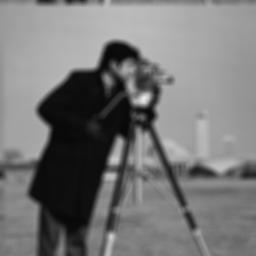
\includegraphics[width=0.30\textwidth]{question6/1_cam_blur}
	}
	\subfigure[Image reconstructed using blur inverse; PSNR +251.54dB]{
	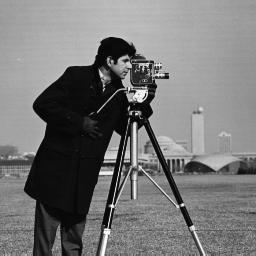
\includegraphics[width=0.30\textwidth]{question6/1_cam_unblur}
	}
	\caption{The base cameraman image has been degraded using a disk blur filter with a radius of 4.}
\end{figure}

\clearpage
\subsection{Noise and image restoration using the inverse}
Gaussian noise has been added to the image after it has been blurred. Applying the inverse blur operation may not be able to restore the image to it's original state.

\begin{figure}[ht]
\centering
	\subfigure[Blurred image; PSNR +16.90]{
	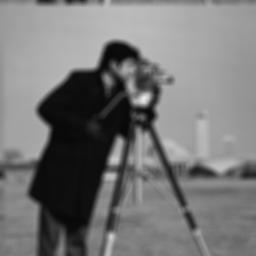
\includegraphics[width=0.30\textwidth]{question6/1_cam_blur}
	}
	\subfigure[Gaussian noise, $\sigma^2$=0.002; PSNR +16.50]{
	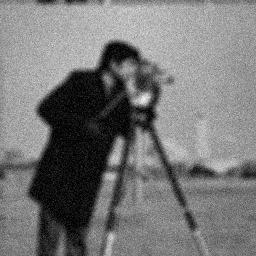
\includegraphics[width=0.30\textwidth]{question6/2_cam_blur_noisy}
	}
	\subfigure[Image reconstructed using blur inverse; PSNR -35.24dB]{
	
\includegraphics[width=0.30\textwidth]{question6/2_cam_unblur_noisy}
	}
\end{figure}


\subsubsection{Compare the restored image with the restored image from the previous step. How does the restored
image and the PSNR differ from the previous restored image? Is it better or worse? Why?}

This restored image looks nothing like the original image. While the blurred images with and without noise appear very similar and have very similar PSNR values; the addition of a small amount of noise prevents inverse filtering from working properly. Adding Gaussian noise will change the Fourier domain representation of the image sufficiently that the inverse operation is unable to recover the original image.

\subsubsection{Can you draw any conclusions about inverse filtering when applied to noise degraded images?}

Inverse filtering applied to noise degraded images is unable to recover the original image, as even small amounts of noise alter the Fourier domain representation of the image sufficiently so that the original image cannot be recovered.


\subsection{Using the Wiener filter for recovering noisy images}

The Wiener filter is able to compensate for the noise present in a degraded image, and reduces the strength of the inverse filter across the image to prevent over-accommodating noise.

\begin{figure}[ht]
\centering
	\subfigure[NSR=0.001; PSNR +5.11dB]{
	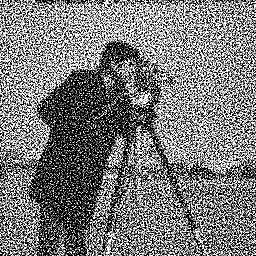
\includegraphics[width=0.30\textwidth]{question6/3_cam_wnr0_001}
	}
	\subfigure[NSR=0.01; PSNR +13.89dB]{
	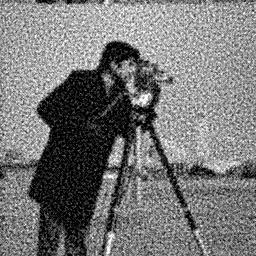
\includegraphics[width=0.30\textwidth]{question6/3_cam_wnr0_01}
	}
	\subfigure[NSR=0.05; PSNR +16.00dB]{
	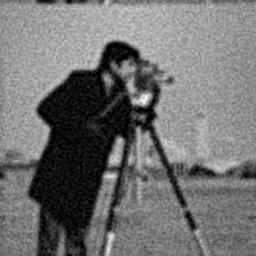
\includegraphics[width=0.30\textwidth]{question6/3_cam_wnr0_05}
	}
	
	\subfigure[NSR=0.1; PSNR +16.16dB]{
	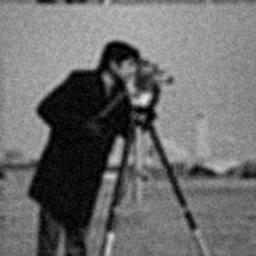
\includegraphics[width=0.30\textwidth]{question6/3_cam_wnr0_10}
	}
	\subfigure[NSR=0.2; PSNR +15.66dB]{
	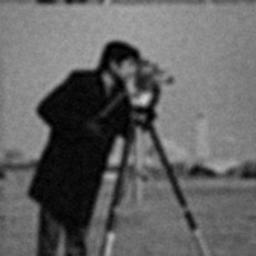
\includegraphics[width=0.30\textwidth]{question6/3_cam_wnr0_20}
	}
	\subfigure[NSR=0.4; PSNR +14.05dB]{
	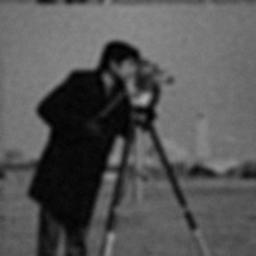
\includegraphics[width=0.30\textwidth]{question6/3_cam_wnr0_40}
	}
	\caption{Wiener filtering with various NSR. As NSR $\rightarrow$0, Wiener filtering becomes normal inverse filtering.}
\end{figure}


\subsubsection{Compare the restored image with the restored image from the previous step. How does the restored image and the PSNR differ from the previous restored image? Is it better or worse? Why? Explain it in context with the concept behind Wiener filtering.}

The restored image using the Wiener filter is much closer to the original (using NSR=0.1 as the best one) than the straight inverse filtering. Wiener filtering attenuates various frequencies when applying an inverse filter. As the noise in the image is relatively flat across all frequencies, the noise to signal ratio is approximated by a constant.

The Wiener filtering can be explained as blending the distorted image with noise with the inverse of the distorted image with noise. By reducing the inverse component, the issue of noise in deconvolution can be reduced.

\subsubsection{Can you draw any conclusions about Wiener filtering when applied to noise degraded images?}

Wiener filtering is able to accommodate noise when attempting to solve the noise problem inherent in deconvolution. The NSR, if unknown, must be carefully chosen in order to to get a good result.

\appendix
\newpage

% -------- Bibliography --------
%\addcontentsline{toc}{chapter}{\hspace{13pt} References}
\bibliography{refs}

\end{document}  